Para este teorema, la hipótesis de convergencia uniforme es clave. Veremos a continuación como en general, el teorema no se cumple para la convergencia puntual.

\begin{ejem}
    Consideremos la siguiente sucesión de funciones sobre $D = [0,1]$:
    
    \[
    f_{n-1}(x) = \begin{cases}
                 2n \quad x \in (1/n, 2/n) \\
                 0  \quad \text{si no}
             \end{cases}
    \]
    
    \noindent con $n \geq 2$.
    
    Al analizar las gráficas, estas son muy parecidas a las de \ref{ejem:cp}, y nos daremos cuenta de que la gráfica tenderá a cero. Entonces
    
    \[
    \limtoinfty{n}{f_n(x)} = f(x) \quad \text{donde $f(x) \equiv 0$ para cada $x \in [0,1]$}
    \]
    
    Pero
    
    \[
    \int_0^1 f_n(x)dx = \int_{\frac{1}{n}}^{\frac{2}{n}} 2ndx = 2
    \]
    
    Por lo tanto $\limtoinfty{n}{\int_0^1 f_n(x)dx} = 2$ y $\int_0^1 \limtoinfty{n}{f_n(x)}dx = 0$.
\end{ejem}

\begin{cor}
    Sea $\sucinf{f}{n}$ una sucesión de funciones integrables en $[a,b]$, y supongamos que $\sumtoinfty{n=1}{f_n}$ c.u. Entonces
    
    \[
    \intab \left(\sumtoinfty{n=1}{f_n(x)}\right)dx = \sumtoinfty{n=1}{\intab f_n(x)dx}
    \]
\end{cor}

\begin{proof}
    Como $\sucinf{f}{n}$ son integrables Riemann-integrables, entonces por las propiedades de la integral de Riemann, $\sucinf{S}{N}$ son integrables. Como $\sumtoinfty{n=1}{f_n}$ c.u entonces existe $f$ tal que
    
    \[
    \limtoinfty{N}{S_N} = f \quad \text{uniformemente}
    \]
    
    Entonces
    
    \[
    \limtoinfty{N}{\intab S_N(x)dx} = \intab f(x)dx
    \]
    
    Y en conclusión,
    
    \[
    \intab \left(\sumtoinfty{n=1}{f_n(x)}\right)dx = \sumtoinfty{n=1}{\intab f_n(x)dx}
    \]
    
    Así, queda demostrado.
\end{proof}

\begin{ejem}
    Consideremos la siguiente sucesión sobre $D = [0,1]$: $f_n(x) = x^n$ con $n \geq 0$. En el ejemplo \ref{ej:x^n} vimos que
    
    \[
    \sumtoinfty{n=0}{x^n} = \frac{1}{1-x} \quad \text{para cada $x \in [0,1]$}
    \]
    
    Consideremos un $r \in [0,1]$ tal que $x < r$. Entonces
    
    \[
    \left| \sumtoinfty{n=0}{x^n} \right| \leq \sumtoinfty{n=0}{|x^n|} < \sumtoinfty{n=0}{r^n} \qquad \footnotemark
    \]\footnotetext{Como ejercicio, se plantea lo siguiente:
    
    \begin{ejer}
        Demostrar que $\left| \sumtoinfty{n=0}{x^n} \right| \leq \sumtoinfty{n=0}{|x^n|}$.
    \end{ejer}}
    
    Ahora, tenemos una serie numérica $\sumtoinfty{n=0}{r^n}$ que converge a $\frac{1}{1-r}$, y por el teorema \ref{teo:wei}, nos queda que $\sumtoinfty{n=0}{x^n}$ converge. Luego, podemos intercambiar integrales por series gracias al corolario que recién establecimos. Así, sea $y \in (0, r)$,
    
    \[
    -\ln(1-y) = \int_0^y \frac{dx}{1-x} = \int_0^y \left( \sumtoinfty{n=0}{x^n}\right)dx = \sumtoinfty{n=0}{\int_0^y x^ndx} = \sumtoinfty{n=0}{\frac{y^{n+1}}{n+1}}
    \]
    
    De esta forma, hemos obtenido el desarrollo en series de $-\ln(1-y)$. De la misma manera podremos obtener el desarrollo en series de muchas funciones elementales.
\end{ejem}

\begin{teo}
    Sea $\sucinf{f}{n} \subset C'[a,b]$\marginfootnote{Recordemos que $C'$ quiere decir que:
    
    \begin{enumerate}
        \item $f_n: [a,b] \rightarrow \R$.
        \item $f_n$ son continuas.
        \item $f'_n$ son continuas.
    \end{enumerate}}. Supongamos que
    
    \begin{itemize}
        \item $f'_n \xrightarrow[n \to \infty]{\text{c.u}} g$.
        \item $f_n \xrightarrow[n \to \infty]{\text{c.p}} g$.
    \end{itemize}
    
    Entonces $f_n \xrightarrow[n \to \infty]{\text{c.u}} f$ y $f' = g$.
\end{teo}

\begin{proof}
    Demostremos ambos puntos en orden:
    
    \begin{itemize}
        \item Por el 2TFC, dados $m,n \in \N$, $x \in [a,b]$, entonces
    
        \[
        f_n(x) - f_m(x) = \int_a^x (f_n - f_m)'(t)dt + (f_n - f_m)(a)
        \]
        
        Luego
        
        \begin{equation}\label{eq:suc1}
            \norma{f_n - f_m} = \sup_{x \in D} \left| f_n(x) - f_m(x) \right| \leq (b-a)\norma{(f_n - f_m)'} + \left| (f_n - f_m)(a) \right| \quad \footnotemark
        \end{equation}\footnotetext{Se sustituye lo que está en la expresión anterior por lo que tenemos en la norma, y se desarrolla para llegar a ese resultado.}
        
        Por otro lado, como $f'_n$ c.u, entonces es fuertemente Cauchy, y además $\limtoinfty{n}{f_n(a)} = f(a)$ por la c.p de $f_n$. Entonces dado $\varepsilon > 0$, existe un $N_1 \in \N$ tal que
        
        \[
        \norma{(f_n - f_m)'} < \frac{\varepsilon}{2(b-a)}
        \]
        
        \noindent y además, existe un $N_2 \in \N$ tal que
        
        \[
        \left| (f_n - f_m)(a) \right| < \frac{\varepsilon}{2}
        \]
        
        \noindent si $n, m \in \N$ tales que $n, m \geq N_0 = \max(N_1, N_2)$.
        
        Ahora, por \ref{eq:suc1} tenemos que
        
        \[
        \norma{f_n - f_m} \leq (b-a)\norma{(f_n - f_m)'} + \left| (f_n - f_m)(a) \right| < \frac{\varepsilon(b-a)}{2(b-a)} + \frac{\varepsilon}{2} = \varepsilon
        \]
        
        De esta forma, dado $\varepsilon > 0$ entonces existe un $N_0$ tal que si $n, m \geq N_0$ entonces $\norma{f_n - f_m} < \varepsilon$. En conclusión, $\sucinf{f}{n}$ cumple la condición de Cauchy, por lo tanto $f_n \xrightarrow[]{\text{c.u}} f$.
        
        \item Por el 2TFC, tenemos que para cada $n \in \N$,
        
        \[
        f_n(x) = \int_a^x f'_n(t)dt - f_n(a)
        \]
        
        De esta manera,
        
        \begin{gather*}
            f(x) = \limtoinfty{n}{f_n(x)} = \limtoinfty{n}{\left[ \int_a^x f'_n(t)dt - f_n(a) \right]} = \limtoinfty{n}{\int_a^x f'_n(t)dt} - \limtoinfty{n}{f_n(a)} \\
            = \int_a^x [\limtoinfty{n}{f'_n(t)}]dt - f(a) = \int_a^x g(t)dt - f(a)
        \end{gather*}
        
        Nuevamente, por el 1TFC lo anterior implica que $f'(x) = g(x)$.
    \end{itemize}
    
    Así, quedan demostrados ambos puntos.
\end{proof}

\begin{cor}\label{cor:poderosisimo}
    Sea $\sucinf{f}{n} \subset C'[a,b]$ tales que:
    
    \begin{enumerate}
        \item $\sumtoinfty{n=1}{f_n}$ c.p.
        \item $\sumtoinfty{n=1}{f'_n}$ c.u.
    \end{enumerate}
    
    Entonces $\sumtoinfty{n=1}{f_n}$ c.u y además
    
    \[
    \left( \sumtoinfty{n=1}{f_n(t)} \right)' = \sumtoinfty{n=1}{f'_n(x)} \quad \footnotemark
    \]\footnotetext{Como ejercicio queda la demostración del corolario \ref{cor:poderosisimo}. La demostración se logra haciendo el mismo argumento que en el teorema anterior, pero definiendo $S_N = f_1 + \dots + f_N$.}
\end{cor}

\subsection{Teorema de Stone-Weierstrass}

\begin{teo}[Stone-Weierstrass]
    Sea $f \in C[a,b]$, entonces existe una sucesión $\sucinf{P}{n}$ de polinomios en $[a,b]$ tal que $\norma{P_n - f} \xrightarrow[n \to \infty]{} 0$.
\end{teo}

\begin{proof}
    Como primera consideración, en lugar de realizar la demostración en $[a,b]$, la realizaremos en $[0,1]$, podemos hacer esto debido a que si consideramos una función $p(x): [a,b] \rightarrow [0,1]$ tal que
    
    \[
    p(x) = \frac{x-a}{b-a}
    \]
    
    \noindent entonces podemos tomar una composición $p \circ f$, donde $f$ está definida en $[a,b]$.
    
    \begin{marginfigure}
        \centering
        \begin{tikzpicture}
            \begin{axis}[
                axis x line = bottom,
                axis y line = left,
                domain=0:1.1,
                width=5cm,
                height=5cm,
                clip=false,
                xtick=\empty,
                ytick=\empty,
                every axis x label/.style={at={(ticklabel cs: 0.95,0)},
                anchor=north},
                every axis y label/.style={at={(ticklabel cs: 0.95,0)},
                anchor=north east},
                xlabel=$x$,
                ylabel=$y$,
                ]
                \addplot [mark=none, blue, smooth] coordinates { (0,0.5) (0.1,0.4) (0.25, 0.2) (0.6,0.6) (0.8,0.3) (1,0.4) };
                \addplot [mark=*, red] coordinates { (0,0.5) (1,0.4) };
                \node[] at (-13,295) {\footnotesize $f(0)$};
                \node[] at (115,200) {\footnotesize $f(1)$};
            \end{axis}
        \end{tikzpicture}
        \label{fig:stnwei1}
        \caption{\footnotesize Aquí describimos la situación que tenemos en la demostración. Tenemos $f(x)$ como la línea azul, y $L(x)$ como la línea roja.}
    \end{marginfigure}
    
    La otra consideración es que $f(0) = f(1) = 0$. Esto lo podemos hacer porque al tomar la recta $L(x)$ que pasa por $f(0)$ y $f(1)$, entonces
    
    \[
    L(x) = (f(1) - f(0))x - f(0)
    \]
    
    \noindent definamos entonces $h(x) = f(x) - L(x)$. Luego, $h(1) = h(0) = 0$. Lo que hemos hecho es transladar la función $f$, obteniendo una nueva función $h(x)$. De esta manera podemos tomar $f(1) = f(0) = 0$.
    
    Sean para $n \in \N$
    
    \[
    K_n(t) = \begin{cases}
        \dfrac{(1-t^2)^n}{C_n}& \quad \text{si} \quad |t| \leq 1 \\
        0& \quad \text{si} \quad |t| > 1
    \end{cases}
    \]
    
    \noindent donde $\displaystyle C_n = \int_{-1}^1 (1-t^2)^ndt$. Como $(1-t^2)^n$ es una función acotada, la integral dará como resultado un valor finito y positivo (ya que $|t| \leq 1$).\marginfootnote{Estos valores se llaman los núcleos de Landau.}
    
    \begin{marginfigure}
        \centering
        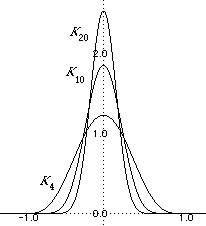
\includegraphics[scale=0.7]{img/landau.png}
        \label{fig:stnwei1}
        \caption{\footnotesize Aquí están representados los núcleos de Landau para algunos valores de $n$.}
    \end{marginfigure}
    
    Sea $z_n(t) = (1-t^2)^n$,
    
    \[
    z_n(-t) = (1-(-t)^2)^n = (1-t^2)^n = z_n(t)
    \]
    
    Por lo tanto, es una función par. Luego
    
    \[
    C_n = \int_{-1}^1 (1-t^2)^ndt = 2\int_0^1 (1-t^2)^ndt \geq 2\int_0^1 (1-t)^ndt = \frac{2}{n+1}
    \]
    
    Por otro lado, si definimos
    
    \[
    P_n(x) = \int_{\R} f(t)K_n(x-t)dt
    \]
    
    Lo primero que podemos notar es que $P_n$ son polinomios, porque $K_n(x-t)$ lo son. Esto es verificable gracias al binomio de Newton. Estimemos entonces cuánto vale $|P_n(x) - f(x)|$
    
    \[
    |P_n(x) - f(x)| = \left| \int_{\R} (f(x) - f(t))K_n(x-t)dt \right|
    \]
    
    \noindent ya que el valor de la integral de los $K_n$ es igual a $1$ \marginfootnote{Esto es porque
    
    \[
    \int_{-1}^1 K_n(t)dt = \frac{1}{C_n} \int_{-1}^1 (1-t^2)^ndt = 1
    \]}. Continuamos desarrollando
    
    \[
    \left| \int_{\R} (f(x) - f(t))K_n(x-t)dt \right| \leq \left| \int_{\R} (f(x) - f(t))\right| K_n(x-t)dt
    \]
    
    Hacemos ahora cambio de variable $u = x-t$. Entonces, lo anterior nos queda como
    
    \[
    \left| \int_{\R} (f(x-u) - f(x))\right| K_n(u)du
    \]
    
    Como $f$ es continua en $[0,1]$, el cual es compacto, entonces $f$ es uniformemente continua. Entonces dado $\varepsilon > 0$, existe un $\delta > 0$ tal que
    
    \begin{equation}\label{eq:stnwei1}
        \text{si} \quad |x-x-u| < \delta \implies |f(x) - f(x-u)| < \varepsilon
    \end{equation}
    
    Entonces, reescribiendo lo que teníamos antes, y separando la integral tenemos que
    
    \begin{gather}\label{eq:stnwei2}
        |P_n(x) - f(x)| \leq \notag \\
        \int_{|u| < \delta/2} \left|f(x-u) - f(x)\right|K_n(u)du + \int_{\delta/2 < |u| < 1} \left|f(x-u) - f(x)\right|K_n(u)du
    \end{gather}
    
    Por un lado, si $|u| < \delta/2$ y se cumple la hipótesis de continuidad, por \ref{eq:stnwei1} tendremos que
    
    \[
    \int_{|u| < \delta/2} \left|f(x-u) - f(x)\right|K_n(u)du \leq \varepsilon \int_{-1}^1 du = \varepsilon
    \]
    
    Y por el otro lado, como $K_n$ son funciones continuas y decrecientes en el intervalo $[\delta/2, 1]$, entonces para $\delta/2 < |u| < 1$, el máximo valor que pueden tomar es $K_n(\delta/2)$. Luego
    
    \begin{gather*}
        \int_{\delta/2 < |u| < 1} \left|f(x-u) - f(x)\right|K_n(u)du \leq K_n(\delta/2)\int_{\delta/2 < |u| < 1} \left|f(x-u) - f(x)\right|du \leq \\
        K_n(\delta/2)\int_{\delta/2 < |u| < 1} 2\norma{f}du = K_n(\delta/2)(2\norma{f})\int_{\delta/2 < |u| < 1}du \leq \\
        K_n(\delta/2)(2\norma{f})\int_{0 < |u| < 1}du = K_n(\delta/2)2\norma{f}
    \end{gather*}
    
    \noindent como los $K_n$ son integrables, conforman una sucesión que converge a cero al hacer $n \rightarrow \infty$. Entonces la expresión $\int_{\delta/2 < |u| < 1} \left|f(x-u) - f(x)\right|K_n(u)du$ puede hacerse tan pequeña como queramos.
    
    De esta forma, retomando lo que teníamos en \ref{eq:stnwei2}
    
    \begin{gather*}
        |P_n(x) - f(x)| < \varepsilon + 0 = \varepsilon \implies \\
        |P_n(x) - f(x)| \xrightarrow[n \to \infty]{} 0 \quad \forall x \in [0,1]
    \end{gather*}
    
    \noindent como el límite es igual a cero cuando $n$ tiene a infinito, pero no depende de $x$, podemos concluir que
    
    \[
    \norma{P_n - f} \xrightarrow[n \to \infty]{} 0
    \]
    
    De esta forma, queda demostrado el teorema.
\end{proof}